
\documentclass[20pt]{beamer}

\usepackage[ngerman,english]{babel}
\usepackage{tikz}
\usepackage[normalem]{ulem}
\geometry{paperwidth=10in, paperheight=7.5in}
\usepackage{animate}
\newcommand{\dd}{\; \mathrm{d}}
\usepackage[utf8]{inputenc}

%\usepackage[mpidr]{./mpidr/beamerthemeMPIDR}


%%%%%%%%%%%%%%%%%%%%%%%%%%%%%%%%%%%%%%%%%%%%%%%%%%%%%%%%%%%%%%%%%%%%%%%%%%%%%%
% Title Page
%%%%%%%%%%%%%%%%%%%%%%%%%%%%%%%%%%%%%%%%%%%%%%%%%%%%%%%%%%%%%%%%%%%%%%%%%%%%%%%

%\title[HLE, mortality and morbidity]{~~~Healthy Life Expectancy,\\~~~ Mortality,
%\\~~~and Age Prevalence of Morbidity}
%\hspace{10cm}
%\small
%\subtitle{Tim Riffe, Alyson van Raalte, Maarten J. Bijlsma}
%\institute[PAA 2016]{MPIDR, Rostock, Germany}
%\date[]{\scriptsize April 2, 2016}

%%	the institute's logo
%\renewcommand{\mylogo}{\includegraphics[width=\textwidth]{beamerstrip.pdf}}
%\usepackage{color}
%\definecolor{mygray}{rgb}{0.8,0.8,0.8}

%\defbeamertemplate{description item}{align left}{\insertdescriptionitem\hfill}
%%	should be the very last package to be loaded
\usepackage{hyperref}
\usefonttheme{serif} 
\begin{document}
%%	titlepage - fixed frame:
%%	========================

\begin{frame}[plain]
	%\titlepage
	\vspace{-4.4cm}
 \centerline{\includegraphics[scale=.16]{beamerstrip.pdf}}

	
	\huge
	\vspace{1em}
	
	Healthy Life Expectancy, Mortality, and Age Prevalence of Morbidity \\
	\vspace{1em}
	\large 
	Tim Riffe, Alyson van Raalte, Maarten J. Bijlsma
\end{frame}

%%%%%%%%%%%%%%%%%%%%%%%%%%%%%%%%%%%%%%%%%%%%%%%%%%%%%%%%%%%%%%%%%%%%%%%%%%%%%%%
\section{Introduction}
%%%%%%%%%%%%%%%%%%%%%%%%%%%%%%%%%%%%%%%%%%%%%%%%%%%%%%%%%%%%%%%%%%%%%%%%%%%%%%%

%%%%%%%%%%%%%%%%%%%%%%%%%%%%%%%%%%%%%%%%%%%%%%%%%
%\begin{frame}{Expected life years with disability (DLY)}
\begin{frame}[plain]
\Large
\begin{center}
\only<1>{HLE most often measured by Sullivan method}
\only<2>{$\mathrm{HLE} = \int \ell(x)\left(1-\pi(x)\right)\dd x$}
\only<3>{Ergo \emph{age} patterns}
\end{center}
\end{frame}

\begin{frame}[plain]
\begin{center}
\includegraphics[width=\textwidth]{Figures/AgePatternsMorbidity.png}
\end{center}
Wingard et al. (1989)
\end{frame}
%%%%%%%%%%%%%%%%%%%%%%%%%%%%%%%%%%%%%%%%%%%%%%%%%
\begin{frame}[plain]
\setbeamercovered{transparent}
\Large
\begin{itemize}[<+->]
\item[-] Stock variable, changes slowly (Barendregt et al. 1994)
\item[-] Prevalence can vary by age, time-to-death, lifespan, or combinations of
these things (Riffe et al. 2017).
\item[-] Complicates comparisons of period HLE (or ULE) across
populations with different mortality.
\end{itemize}
\end{frame}
%%%%%%%%%%%%%%%%%%%%%%%%%%%%%%%%%%%%%%%%%%%%%%%%%


%%%%%%%%%%%%%%%%%%%%%%%%%%%%%%%%%%%%%%%%%%%%%%%%%%
% Morbidity as a function of time to death
%%%%%%%%%%%%%%%%%%%%%%%%%%%%%%%%%%%%%%%%%%%%%%%%%%

%%%%%%%%%%%%%%%%%%%%%%%%%%%%%%%%%%%%%%%%%%%%%%%%%%%%%%%%%%%%%%

\begin{frame}[plain]
\begin{center}
 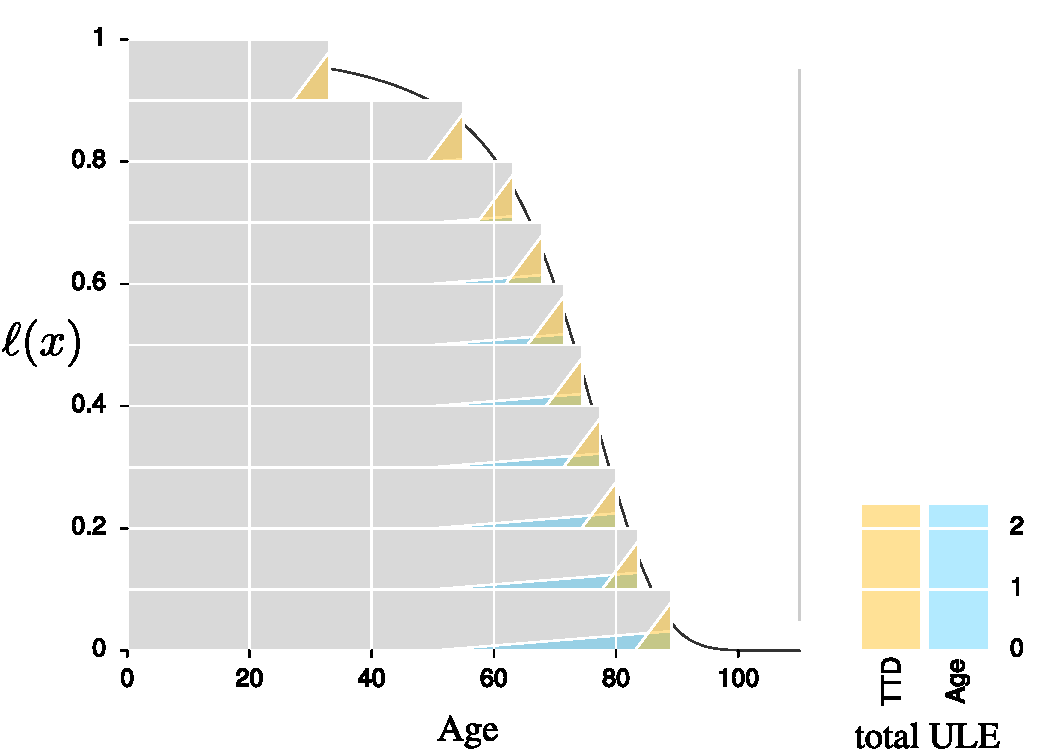
\includegraphics[width=\linewidth]{Figures/Japan1970.pdf}
 %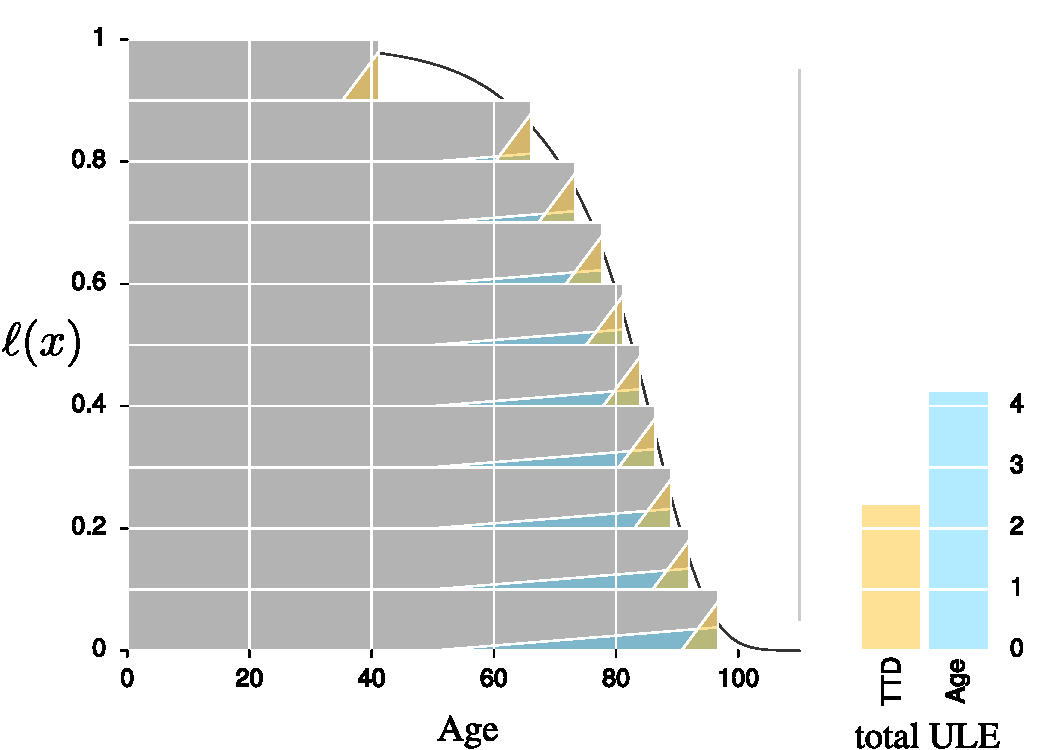
\includegraphics[width=.5\linewidth]{Figures/Japan2010.pdf}
\end{center}
\end{frame}


\begin{frame}[plain]
\begin{center}
 %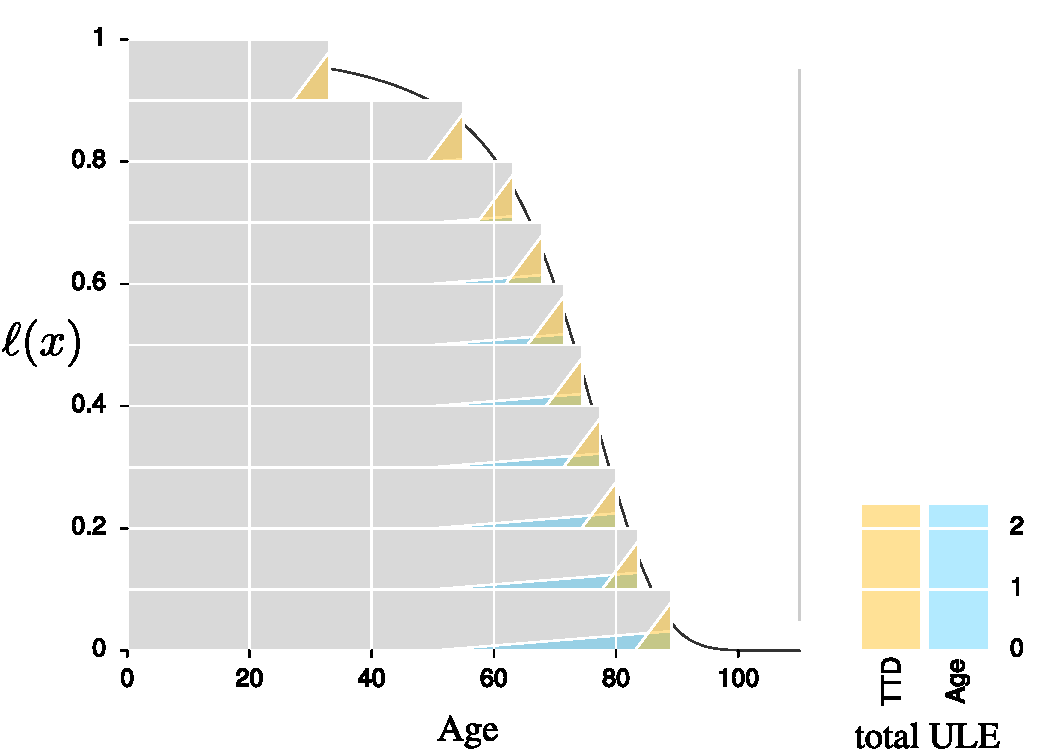
\includegraphics[width=.5\linewidth]{Figures/Japan1970.pdf}
 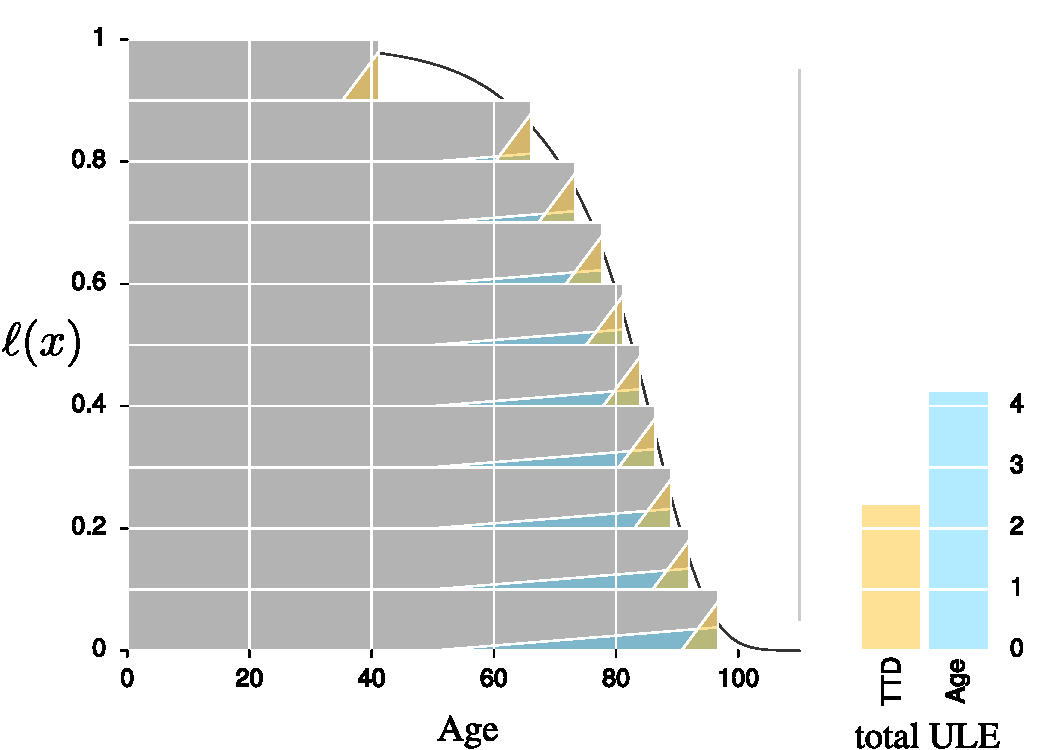
\includegraphics[width=\linewidth]{Figures/Japan2010.pdf}
\end{center}
\end{frame}

\begin{frame}[plain]
\begin{center}
\includegraphics[scale=2]{Figures/Klijs2011.jpg}
\end{center}
Klijs et al. (2011)
\end{frame}

%%%%%%%%%%%%%%%%%%%%%%%%%%%%%%%%%%%%%%%%%%%%%%%%%%%%%%%%%%%%%%%%%%%%%%%%%%%%%%%%%%%%%%%%%%%%%%%
\begin{frame}[plain]
\begin{center}
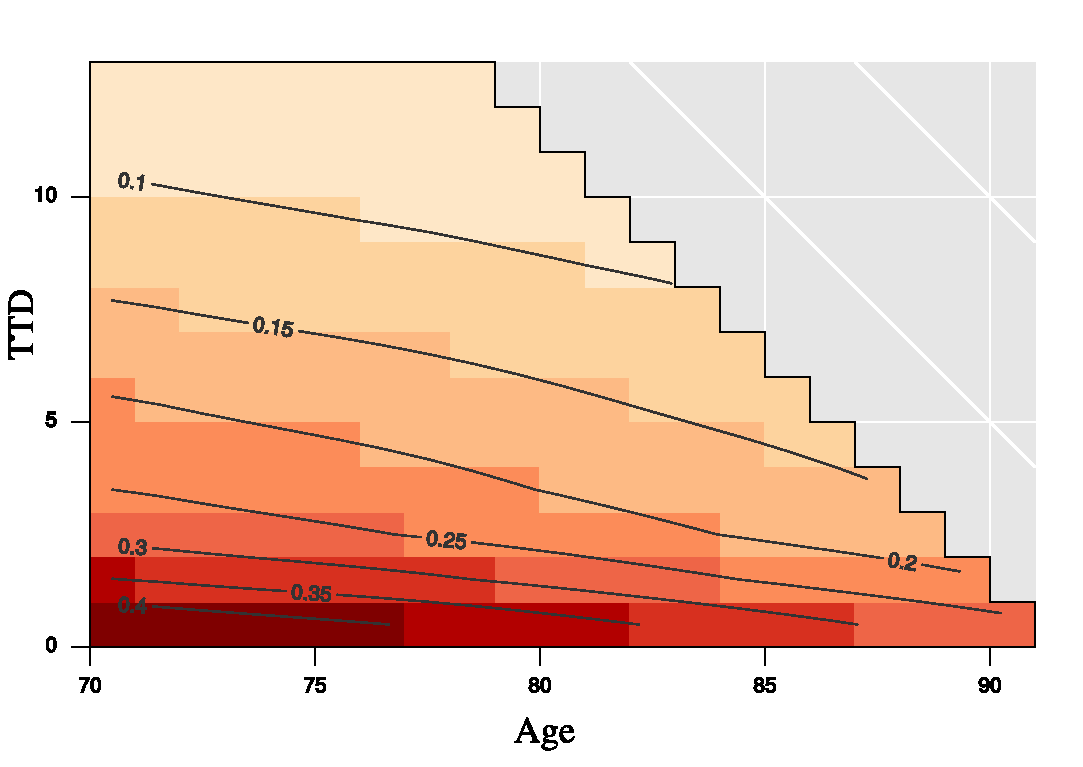
\includegraphics[scale=1.2]{Figures/srhpoor_f_Surf_a.pdf}
\\
\normalsize Prevalence of USA
females (1915-1919 cohort) self-reporting poor health (HRS)
\end{center}
\end{frame}

\begin{frame}[plain]
\begin{center}
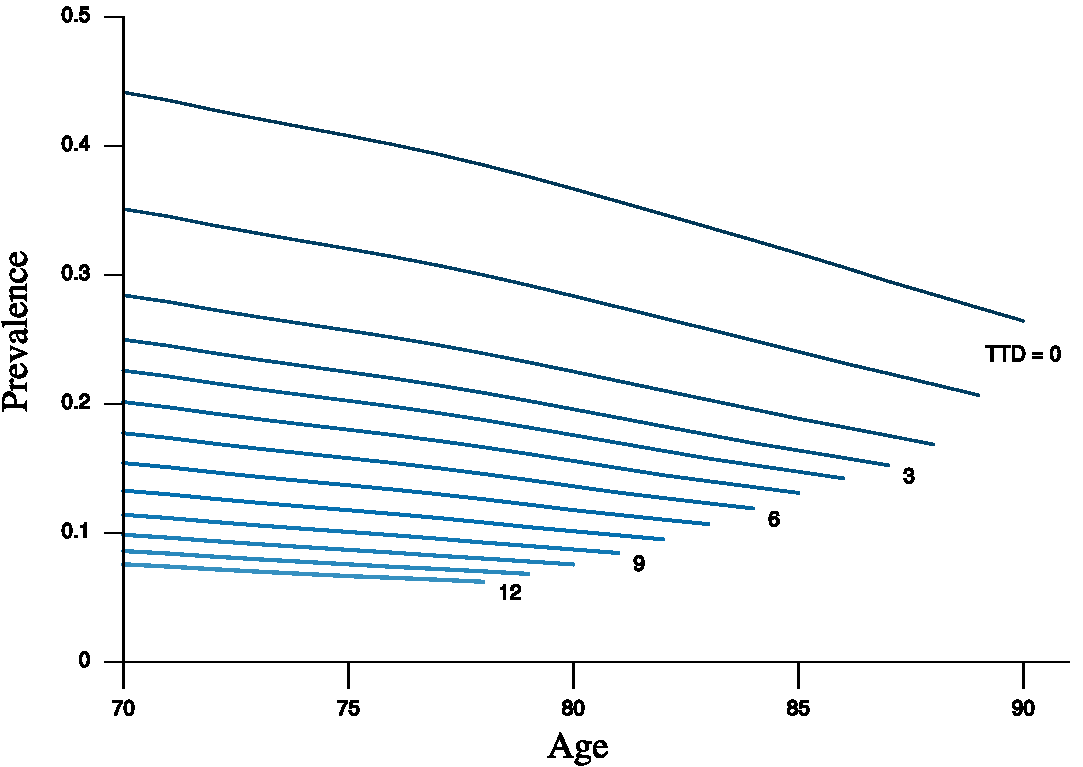
\includegraphics[scale=1.2]{Figures/srhpoor_f_Age_c.pdf}
\end{center}
\end{frame}

\begin{frame}[plain]
\begin{center}
\only<1>{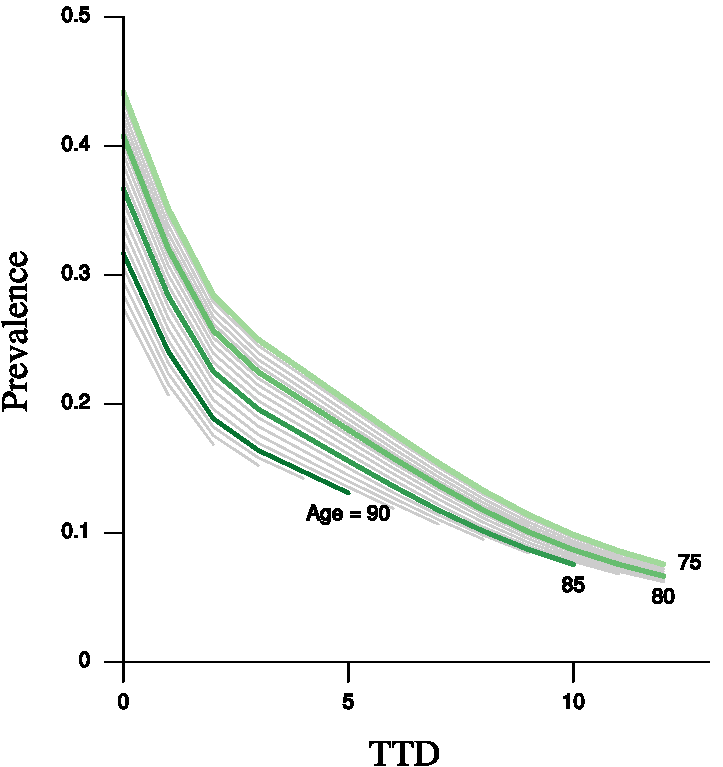
\includegraphics[scale=1.2]{Figures/srhpoor_f_TTD_b.pdf}}
\only<2>{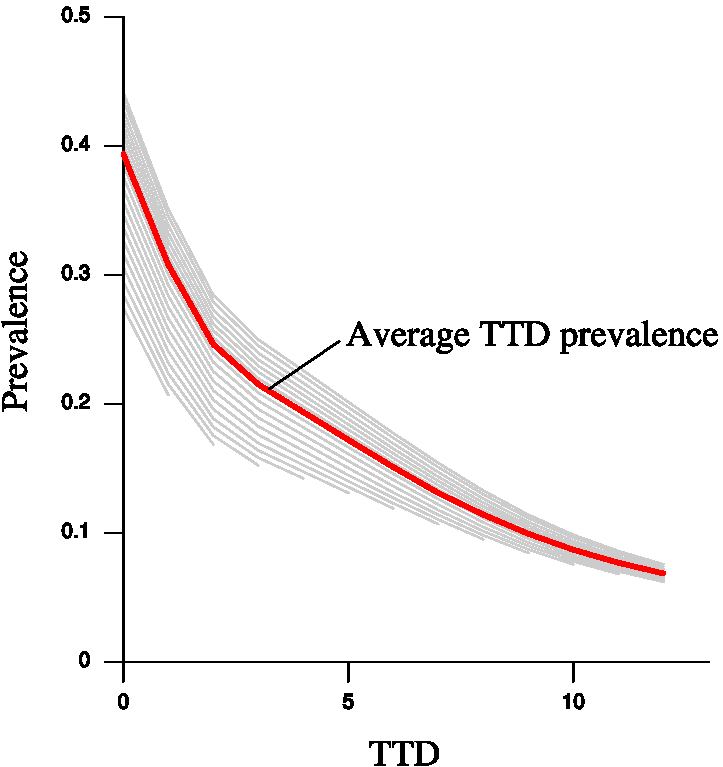
\includegraphics[scale=1.2]{Figures/srhpoor_f_TTD_b2.pdf}}
\end{center}
\end{frame}

%%%%%%%%%%%%%%%%%%%%%%%%%%%%%%%%%%%%%%%%%%%%%%%%%%%%%%%%%%%%%
% How changing mortality affects morbidity prevalence
%%%%%%%%%%%%%%%%%%%%%%%%%%%%%%%%%%%%%%%%%%%%%%%%%%%%%%%%%%%%%%
\begin{frame}[plain]
\Large
\begin{center}
Held constant, time-to-death prevalence moves \emph{with} longevity.
\end{center}
\end{frame}

%%%%%%%%%%%%%%%%%%%%%%%%%%%%%%%%%%%%%%%%%%%%%%%%%%%%%%%%%%%%%%%%%%

\begin{frame}[plain]
\begin{overprint}
\begin{center}
\only<1>{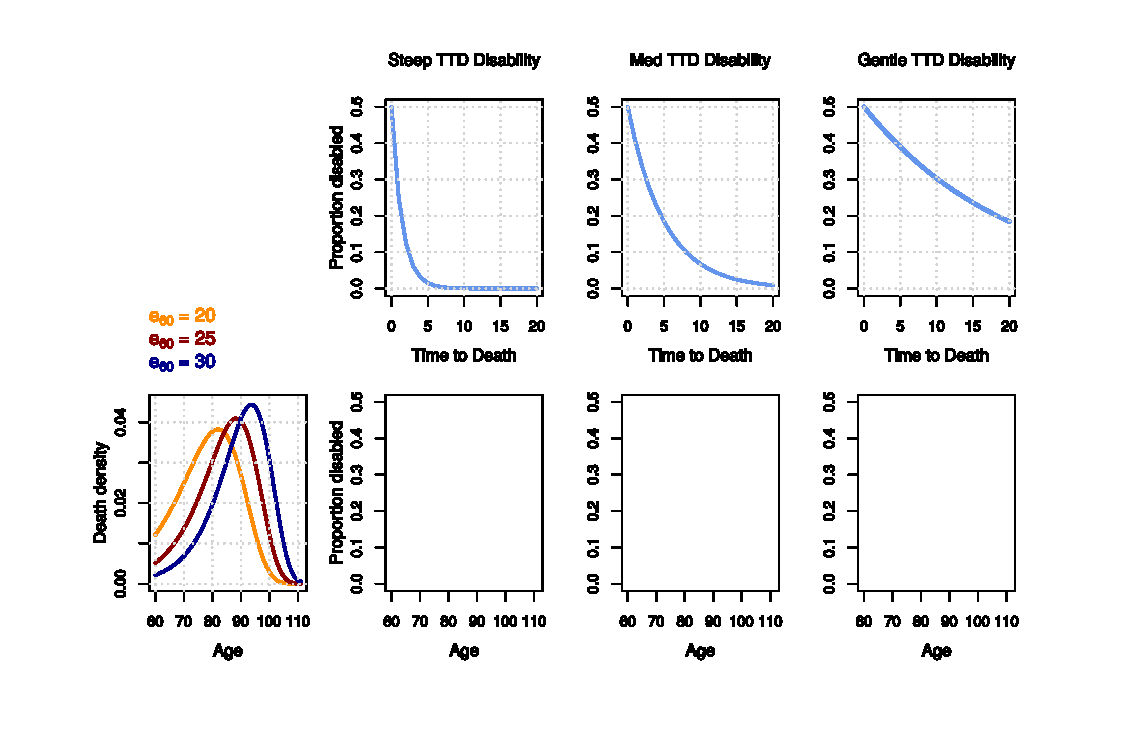
\includegraphics[trim=1cm 0 0 0, clip,width=1.1\linewidth]{Figures/schematic_pres0.pdf}}
\only<2>{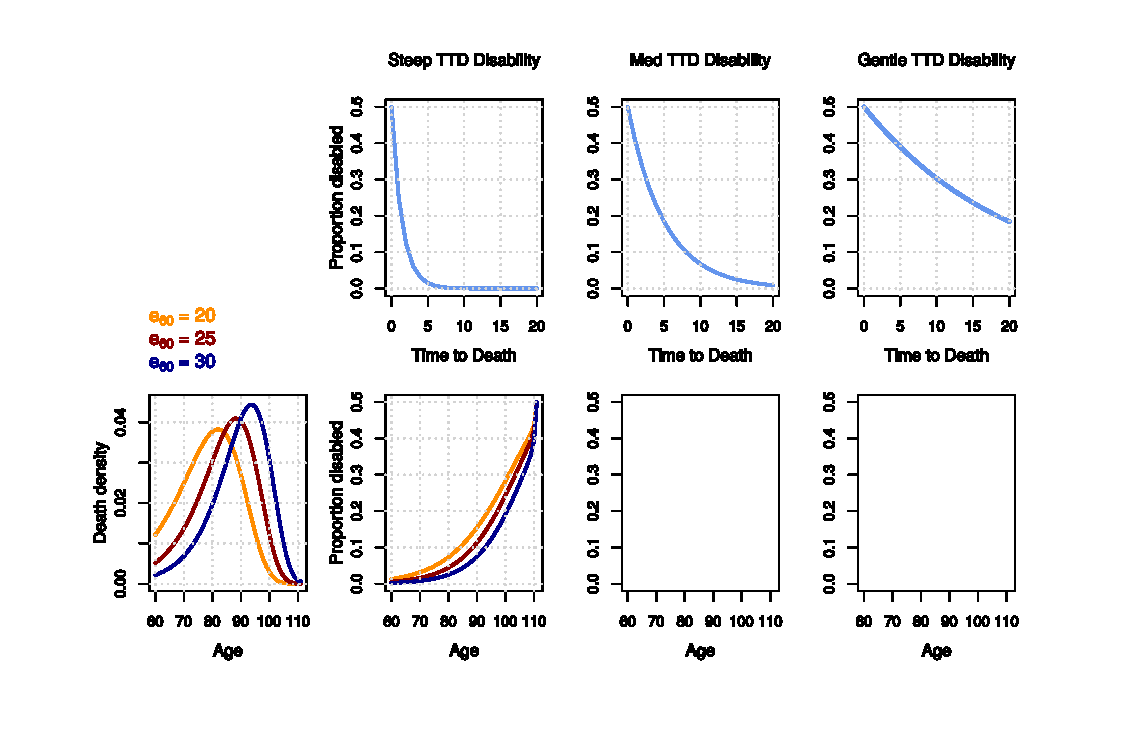
\includegraphics[trim=1cm 0 0 0, clip,width=1.1\linewidth]{Figures/schematic_pres1.pdf}}
\only<3>{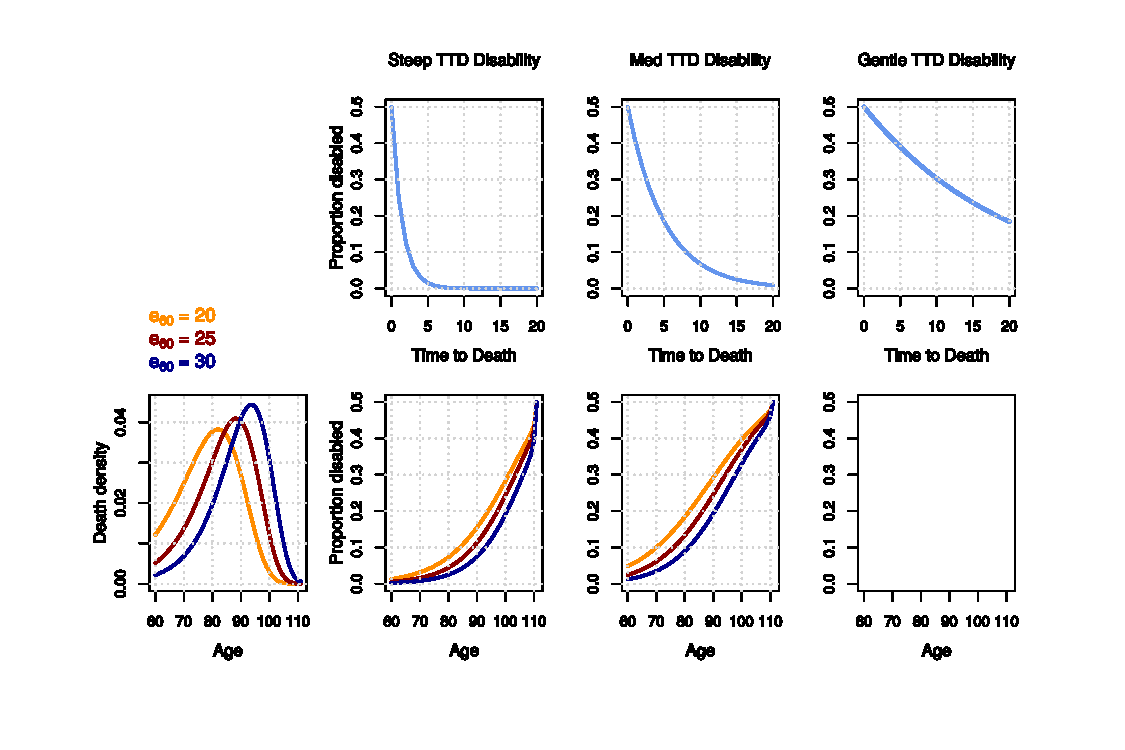
\includegraphics[trim=1cm 0 0 0, clip,width=1.1\linewidth]{Figures/schematic_pres2.pdf}}
\only<4>{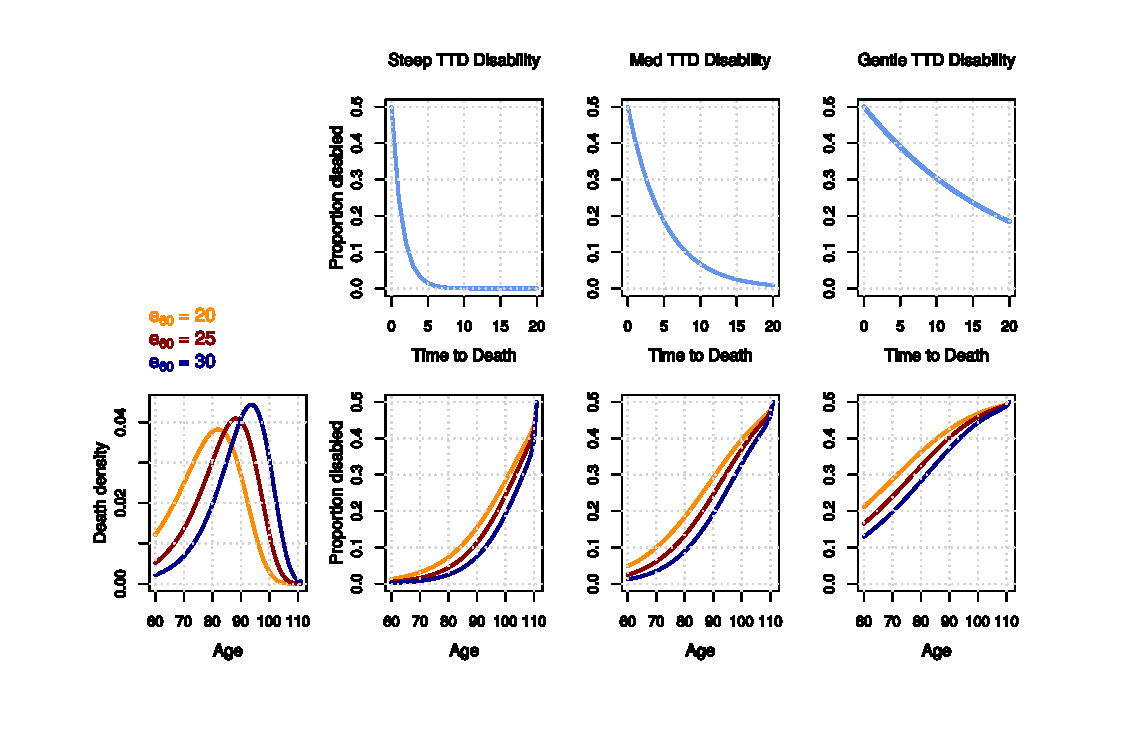
\includegraphics[trim=1cm 0 0 0, clip,width=1.1\linewidth]{Figures/schematic_pres3.pdf}}
\end{center}
\end{overprint}
\end{frame}
%%%%%%%%%%%%%%%%%%%%%%%%%%%%%%%%%%%%%%%%%%%%%%%%%%%%%%%%%%%%%%%%%%

%%%%%%%%%%%%%%%%%%%%%%%%%%%%%%%%%%%%%%%%%%%%%%%%%%%%%%%%%%%%%%%%
% Attributing DLY differences to mortality and morbidity
%%%%%%%%%%%%%%%%%%%%%%%%%%%%%%%%%%%%%%%%%%%%%%%%%%%%%%%%%%%%%%%%

\begin{frame}[plain]
\Large
\begin{center}
\only<1>{ Are differences in HLE (ULE) due to \\mortality or
morbidity?}
\only<2>{Decomposition methods isolate the effects of changes in $\mu_x$ and changes
in $\pi_x$}
\only<3>{Considered as \textit{mortality} and \textit{morbidity} effects (Andreev et al. 2002, Nusselder and Looman 2004)}
\only<4>{Interpretation problem: $\pi_x$ itself \\can change with longevity}
\only<5>{How biased might such decompositions be?}
\end{center}
\end{frame}

%%%%%%%%%%%%%%%%%%%%%%%%%%%%%%%%%%%%%%%%%%%%%%%%%%%%%%%%%%%%%%%%%%
\begin{frame}[plain]
\setbeamercovered{transparent}
\Large
\begin{itemize}[<+->]
\item Estimate empirical TTD profiles for different disabilities (USA HRS, 1905-1930 cohorts)
\item Convert TTD profiles to $\pi_x$ using HMD lifetables
\item Assume all populations stationary
\item Decompose pairwise ULE differences between all populations (1980, 1990, 2000) into \emph{mortality} and \emph{morbidity} components
\item Same for within-population changes over 10-year periods, 1950-2010
\item (By design, all ULE differences due 100\% to mortality)
\end{itemize}
\end{frame}

%%%%%%%%%%%%%%%%%%%%%%%%%%%%%%%%%%%%%%%%%%%%%%%%%%%%%%%%%%%%%%%%%%%%%%%
\begin{frame}[plain]
\begin{center}
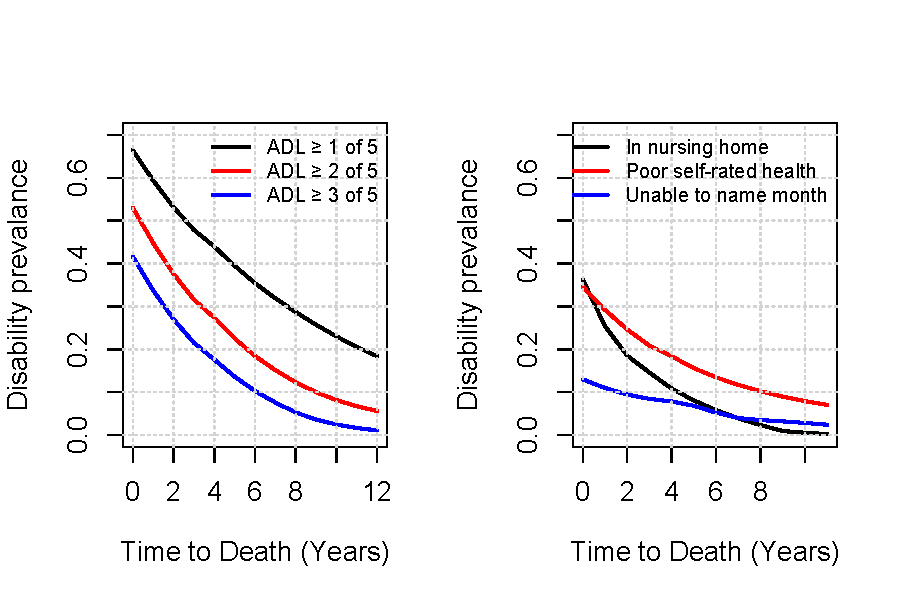
\includegraphics[scale=1.3]{Figures/DisbyTTD_pres.pdf}
\end{center}
\end{frame}
%%%%%%%%%%%%%%%%%%%%%%%%%%%%%%%%%%%%%%%%%%%%%%%%%%%%%%%%%%%%%%%%%%%%%%%

\begin{frame}[plain]
\begin{center}
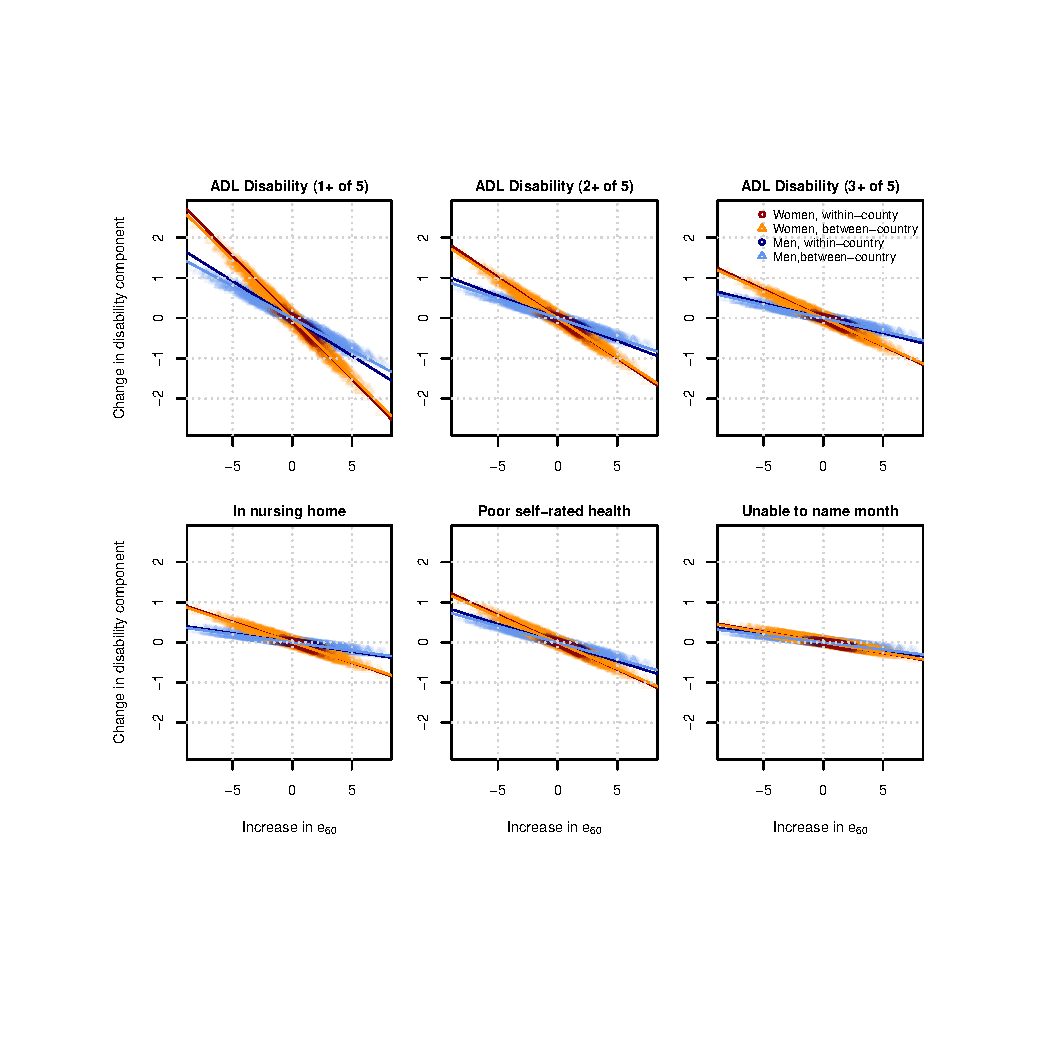
\includegraphics[trim=1cm 0 0 2.5cm, clip, scale=1.3]{Figures/Decomp_2x3.pdf}
\end{center}
\end{frame}
%%%%%%%%%%%%%%%%%%%%%%%%%%%%%%%%%%%%%%%%%%%%%%%%%%%%%%%%%%%%%%%%%%%%%%%%%

\begin{frame}[plain]
\setbeamercovered{transparent}
\Large
\begin{itemize}[<+->]
\item If $e_{60}$ increases by 5 years, up to 1 year of decrease in ULE attributed to disability component could be from decrease in mortality (Female ADL 3+)
\item Different slopes partly from differences in final $\pi_x$ between
disability types and the sexes
\end{itemize}
\end{frame}
%%%%%%%%%%%%%%%%%%%%%%%%%%%%%%%%%%%%%%%%%%%%%%%%%%%%%%%%%%%%%%%%%%%%%%%%%%%%

%%%%%%%%%%%%%%%%%%%%%%%%%%%%%%%%%%%%%%%%%%%%%%%%%%%%%%%%%%%%%
% Conclusion
%%%%%%%%%%%%%%%%%%%%%%%%%%%%%%%%%%%%%%%%%%%%%%%%%%%%%%%%%%%%%%

\begin{frame}[plain]
\setbeamercovered{transparent}
\Large
\begin{itemize}[<+->]
\item TTD prevalence can result from age-patterned transitions (incidence)
\item Modeling prevalence as TTD requires no specification of process
\item Morbidity varies over both age and time-to-death
\end{itemize}
\end{frame}

%%%%%%%%%%%%%%%%%%%%%%%%%%%%%%%%%%%%%%%%%%%%%%%%%%%%%%%%%%%%%%%%%%
\begin{frame}[plain]
\setbeamercovered{transparent}
\Large
\begin{itemize}[<+->]
\item HLE (ULE) important health metrics
\item Difficult to properly interpret period differences 
\item Age patterns of disability can change due to mortality, even if TTD prevalence held constant (dynamic equilibria re Klijs et al. 2011)
\item Could partly explain why mortality levels and disability prevalence are related (Van Oyen et al. 2013, Luy and Minagawa 2014)
\end{itemize}
\end{frame}

%%%%%%%%%%%%%%%%%%%%%%%%%%%%%%%%%%%%%%%%%%%%%%%%%%%%%%

\begin{frame}
\frametitle{Thanks!}
\begin{center}
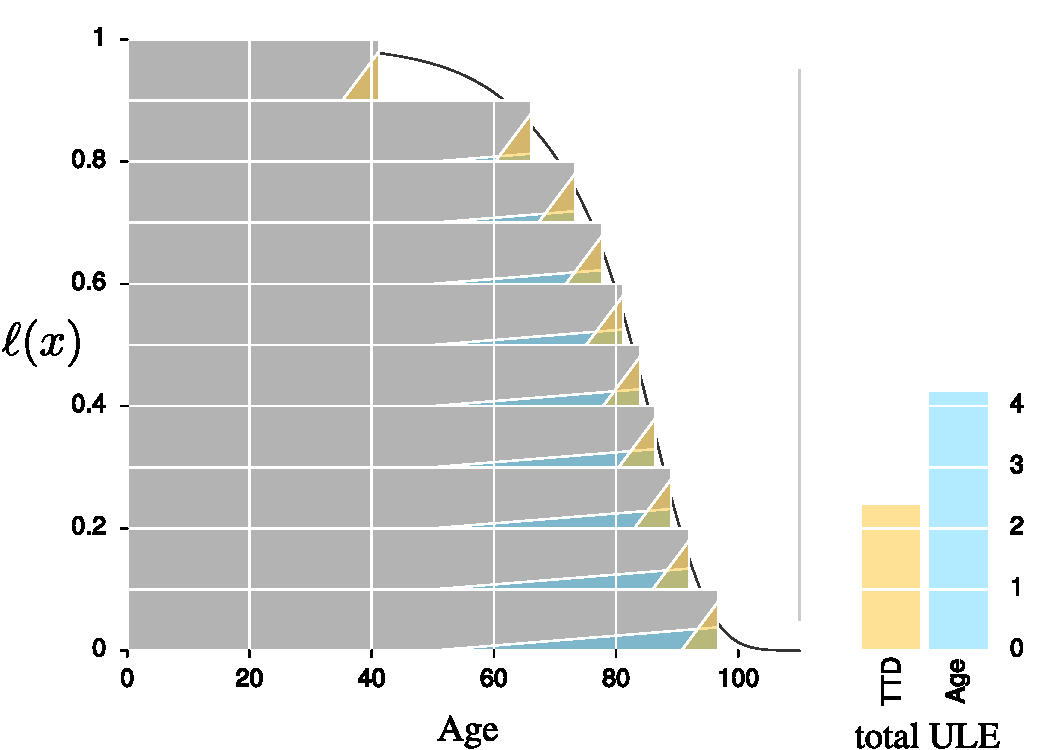
\includegraphics[width=\linewidth]{Figures/Japan2010.pdf}
\end{center}
\end{frame}

%%%%%%%%%%%%%%%%%
\end{document}